%\documentclass[twocolumn,11pt]{article}
\documentclass[11pt]{article}
\usepackage{listings}
\usepackage{amsmath,amsfonts,amssymb,amsthm}
\usepackage[mathscr]{euscript}
\usepackage{verbatim}
\usepackage {tikz}
\usepackage{graphicx,wrapfig}
\usetikzlibrary {positioning}
\usetikzlibrary{shapes}
\usepackage{subcaption}
%\definecolor {processblue}{cmyk}{0.96,0,0,0}

\begin{document}

\title{Branch Back Formalism for Programs}
\author{C. E. Clauson}
\maketitle

\begin{abstract}
We introduce a formula language, called "Branch Back", which is somewhat similar to but also more general than the While programming language which has been defined in literature (source?).  Branch Back is somewhat more general than a programming language, but is rather a class of languages, in which a program is a formula in the language. A term rewrite system-based operational semantics is defined, and the system is shown to be equivalent to more familiar control flow diagrams for computer programs.
\end{abstract}

\section{Introduction}
The motivation of Branch Back starts in the observation that many models and languages for programs are similar in having finite control, but differ in state external to that finite control, the mutations that the state can undergo, and the ways in which that state impacts the evolution of the program.

For example, a pushdown automaton relies on finite control coupled with a pushdown stack.  The control can push letters onto or pop letters off of the stack, and can branch based on the letter on the top of the stack.  A Turing machine, by contrast, relies on an infinite tape with a head.  This state external to the control can be modified by moving the head and writing a letter to the current position, and the control can test the letter currently under the head.

Additional examples can be produced.  What we notice is that the various cases are similar in many respects, but differ in the following:

\begin{itemize}
\item The state space available to the program external to the finite control
\item The set of operations the control can use to modify that state
\item The set of operations the control can use to test the state for the purposes of branching
\end{itemize}

In the examples given above (pushdown automaton, Turing machine) the reader will be familiar with the finite control being described via an edge-weighted graph, where edges describe transitions and are weighted with conditions and state operations.  Program execution consists of transitioning through states beginning at a start state until some end state is reached (referred to later as a \emph{control flow graph}).

Branch Back is a general formula language powerful enough to describe all programs possible in a paradigm with a given (state, mutator set, condition set) triple, while meeting the following goals:

\begin{itemize}
\item An exceedingly simple language definition
\item Having an operational semantics based on a deterministic term rewrite system (i.e. similar to lambda calculus)
\end{itemize}

Branch Back will be shown to meet these criteria.  Proofs will be provided for equivalence between branch back formulas and control flow graphs, with algorithms for interconversion.

The symbol $\mathbb{B}$ will be used to represent the Boolean set, which has the members \texttt{true} and \texttt{false}.

\section{Branch Back}
For a given quintuple $(S, M, C, \delta_{M}, \delta_{C})$, we define the set $BB(S, M, C, \delta_{M}, \delta_{C})$ as a set of formulas, under the following assumptions:

\begin{itemize}
\item Each member of $S$ (state set) is finitely representable (and thus $S$ is at most countably infinite).
\item Each member of $M$ (primitive state mutations) can be represented by a finite formula (and thus $M$ is at most countably infinite).
\item Each member of $C$ (primitive conditions) can be represented by a finite formula (and thus $C$ is at most countably infinite).
\item The function $\delta_{M} : M \times S \rightarrow S$, which dictates how members of $M$ mutate members of $S$, is a computable function. 
\item The function $\delta_{C} : C \times S \rightarrow \mathbb{B}$, which evaluates members of $C$ at given states in $S$, is a computable function.
\end{itemize}

Additionally, we assume that there exists a set $L$, the label set, which is countably infinite.

We now inductively define the program formulas.  A given program formula is always \emph{open in} some (possibly empty) set contained in $L$, \emph{immediately open in} some (possibly empty) set contained in $L$, and also \emph{binds} some (possibly empty) set contained in $L$.  The inductive definition is as follows:

\begin{enumerate}
\item The special formula \texttt{HALT} is a program formula open in $\emptyset$, immediately open in $\emptyset$ and which binds $\emptyset$, where $\emptyset$ is the empty set.
\item For every member $l$ of $L$ there exists a program formula $\texttt{branchback(}l\texttt{)}$ open in $\{l\}$, immediately open in $\{l\}$, and which binds $\emptyset$, where $\{l\}$ is the singleton set containing only $l$.
\item If $m$ is a member of $M$ and $p$ is a program formula open in $L_{O}$, immediately open in $L_{OI}$ and which binds $L_{B}$, then $m\texttt{;}p$ is a program formula open in $L_{O}$, immediately open in $\emptyset$, and which binds $L_{B}$, where \texttt{;} is the \emph{sequencing operator}.
\item If $p_{1}$ is a program formula open in $L_{O,1}$, immediately open in $L_{OI,1}$ and that binds$L_{B,1}$, and $p_{2}$ is a program formula open in $L_{O,2}$, immediately open in $L_{OI,2}$ and that binds $L_{B,2}$, and $c$ is a condition, then \texttt{if} $c$ \texttt{then} $p_{1}$ \texttt{else} $p_{2}$ is a program formula open in $L_{O,1} \cup L_{O,2}$, immediately open in $\emptyset$, and which binds $L_{B,1} \cup L_{B,2}$, under the condition that $L_{O,1}$ and $L_{B,2}$ are disjoint, and $L_{O,2}$ and $L_{B,1}$ are disjoint.
\item If $l$ is a member of $L$, $p$ is a program formula open in $L_{O}$, immediately open in $L_{OI}$, binds $L_{B}$, and $l \notin L_{OI}$, then $\texttt{label(}l\texttt{,} p\texttt{)}$ is a program formula open in $L_{O} \setminus \{l\}$, the set $L_{O}$ with $l$ removed, immediately open in $L_{OI}$ and binds $L_{B} \cup \{l\}$.
\end{enumerate}

\newtheorem*{immedopencontainedinopen}{Theorem}
\begin{immedopencontainedinopen}
If $p$ is a program formula open in $L_{O}$ and immediately open in $L_{OI}$, then $L_{OI} \subseteq L_{O}$.
\end{immedopencontainedinopen}

\begin{proof}
We prove by structural induction.  The base cases are \texttt{HALT} and the various $\texttt{branchback(}l\texttt{)}$ instances, for both of these $L_{OI} = L_{O}$ which implies $L_{OI} \subseteq L_{O}$.

The cases $m\texttt{;}p$ and \texttt{if} $c$ \texttt{then} $p_{1}$ \texttt{else} $p_{2}$ are easily handled since in both $L_{OI} = \emptyset$, which is contained in every set.

To treat $\texttt{label(}l\texttt{,} p\texttt{)}$, we use the inductive hypothesis, which lets us infer that $L_{OI} \subseteq L_{O}$, where $L_{O}$ and $L_{OI}$ are the sets in which $p$ is open and immediately open respectively.  To complete the inductive step we must show that $L_{OI} \subseteq L_{O} \setminus \{l\}$, but this easily follows from the requirement imposed by the inductive definition that $l \notin L_{OI}$.
\end{proof}

We define a program formula to be \emph{closed} if and only if it is open in $\emptyset$.

\newtheorem*{closedimmedopeninempty}{Theorem}
\begin{closedimmedopeninempty}
If $p$ is a closed program formula then it is immediately open in $\emptyset$.
\end{closedimmedopeninempty}

\begin{proof}
By definition, $p$ is open in $\emptyset$, therefore $L_{OI} \subseteq \emptyset$.  But only $\emptyset$ is contained in $\emptyset$, therefore $L_{OI} = \emptyset$.
\end{proof}

We define Branch Back programs to be exactly those program formulas which are closed.

\section{Execution of A Branch Back Program}

From a high level, the effect of executing a branch back program is to change from one state in $S$ to another state in $S$, which will occur exactly if the program terminates, which it may or may not do.

More specifically, execution occurs by forming a new kind of formula, an \emph{eval formula}, and applying term rewrite rules until no more can be applied.

\subsection{Branch Back Substitution for Program Formulas}

Before looking at eval formulas, we will start by presenting a term rewrite rule for program formulas and analyzing the system using the singleton containing that rule.

The rule is:

\begin{description}
\item[BranchBackSubstProg] $\texttt{label(}l\texttt{,} p\texttt{)} \longrightarrow [\texttt{branchback(}l\texttt{)} \mapsto \texttt{label(}l\texttt{,} p\texttt{)}]p$ (where the notation $[x \mapsto y]f$ denotes the formula $f$ with term $x$ everywhere replaced with the term $y$)
\end{description}

In a term rewrite system a formula is said to be \emph{normal} if no rules can be applied to reduce it.

\newtheorem*{branchbacksubstnormals}{Theorem}
\begin{branchbacksubstnormals}
\texttt{HALT}, $\texttt{branchback(}l\texttt{)}$ for all $l \in L$, programs of form $m\texttt{;}p$ and of form \texttt{if} $c$ \texttt{then} $p_{1}$ \texttt{else} $p_{2}$ are exactly the normal formulas in \textbf{BranchBackSubstProg}.
\end{branchbacksubstnormals}

\begin{proof}
The four cases listed are just exactly the cases of program formulas not of the form $\texttt{label(}l\texttt{,} p\texttt{)}$.  But since programs of the form $\texttt{label(}l\texttt{,} p\texttt{)}$ are exactly those to which \textbf{BranchBackSubstProg} can apply, we are done.
\end{proof}

A term rewrite system is said to be \emph{deterministic} if and only if every formula can be reduced to at most one new formula in a single reduction step, or stated equivalently, if $t$, $t'$ and $t''$ are formulas such that $t \rightarrow t'$ and $t \rightarrow t''$, then $t' = t''$.

\newtheorem*{branchbacksubstisdeterministic}{Theorem}
\begin{branchbacksubstisdeterministic}
\textbf{BranchBackSubstProg} is deterministic.
\end{branchbacksubstisdeterministic}

\begin{proof}
Because our system has only one reduction rule, it's a trivial result that for a given formula, at most one reduction rule can be applied to it.  Also, the rule \textbf{BranchBackSubstProg} can only be applied in one way to a given eligible formula, the way being dictated by the $l \in L$ in the \texttt{label()} at the root.
\end{proof}

A term rewrite system is said to be \emph{normalizing} if for every formula at most a finite number of reductions can be applied before reaching a normal form.

\begin{comment}

\newtheorem*{labelsfinite}{Lemma}
\begin{labelsfinite}
The number of labels in a program formula is finite.
\end{labelsfinite}

\begin{proof}
Trivial from either structural induction, or just the property of formulas being finite.
\end{proof}

\end{comment}

\newtheorem*{formofnonnormalbbsp}{Lemma}
\begin{formofnonnormalbbsp}
Every non-normal formula of \textbf{BranchBackSubstProg} has the form $\texttt{label(}l_{n}\texttt{,} ... \texttt{label(}l_{3}\texttt{,} \texttt{label(}l_{2}\texttt{,} \texttt{label(}l_{1}\texttt{,} p\texttt{)}\texttt{)}\texttt{)} ... \texttt{)}$ where $n \geq 0$ and $p$ is some normal formula.
\end{formofnonnormalbbsp}

\begin{proof}
By structural induction.  We show that for every possible formula either it is normal or it is of the form above.

The base cases \texttt{HALT} and $\texttt{branchback(}l\texttt{)}$ for each $l$ in $L$ are trivial since all of these forms are normal.

The inductive step requires showing that if each of $q_{1}$ and $q_{2}$ is either normal or of the above form, then any formula that can be constructed from it in a single step is.  Both $m\texttt{;}q_{1}$ and \texttt{if} $c$ \texttt{then} $q_{1}$ \texttt{else} $q_{2}$ are easily handled because both are normal.  This leaves $\texttt{label(}l_{i}\texttt{,} q_{1}\texttt{)}$, which can't be normal.  We must show that if $q_{1}$ is either normal or of the form above then this expression is of the form above.

But this is immediate.  If $q_{1}$ is normal, then $\texttt{label(}l_{i}\texttt{,} q_{1}\texttt{)}$ is just the case for $n = 1$.  If $q_{1}$ is of the form above for some $n$, then adding an additional level of nesting makes it also of the above form but with $n + 1$.  This covers both cases, completing the inductive proof.
\end{proof}

\newtheorem*{bbspnorecurse}{Lemma}

\begin{bbspnorecurse}
If
$$\texttt{label(}l_{n}\texttt{,}\texttt{label(}l_{n - 1}\texttt{,} ... \texttt{label(}l_{3}\texttt{,} \texttt{label(}l_{2}\texttt{,} \texttt{label(}l_{1}\texttt{,} p\texttt{)}\texttt{)}\texttt{)} ... \texttt{)}\texttt{)}$$ reduces to $$\texttt{label(}l_{n - 1}\texttt{,} ... \texttt{label(}l_{3}\texttt{,} \texttt{label(}l_{2}\texttt{,} \texttt{label(}l_{1}\texttt{,} p'\texttt{)}\texttt{)}\texttt{)} ... \texttt{)}$$ via \textbf{BranchBackSubstProg}, and $p$ is normal, then $p'$ is also normal.
\end{bbspnorecurse}

\begin{proof}
Suppose $p'$ is not normal, then it has the form $\texttt{label(}l_{i}\texttt{,} q\texttt{)}$.  Because by hypothesis $p$ is normal and therefore not of a similar form, it must be the case that $p$ is $\texttt{branchback(}l_{n}\texttt{)}$.

However, this implies that $$\texttt{label(}l_{n}\texttt{,}\texttt{label(}l_{n - 1}\texttt{,} ... \texttt{label(}l_{3}\texttt{,} \texttt{label(}l_{2}\texttt{,} \texttt{label(}l_{1}\texttt{,} p\texttt{)}\texttt{)}\texttt{)} ... \texttt{)}\texttt{)}$$ is not a valid formula.  The reason is that $p$ is immediately open in $\{l_{n}\}$, which means so is $\texttt{label(}l_{1}\texttt{,} p\texttt{)}$ and $\texttt{label(}l_{2}\texttt{,} \texttt{label(}l_{1}\texttt{,} p'\texttt{)}\texttt{)}$ and so on up to $$\texttt{label(}l_{n - 1}\texttt{,} ... \texttt{label(}l_{3}\texttt{,} \texttt{label(}l_{2}\texttt{,} \texttt{label(}l_{1}\texttt{,} p'\texttt{)}\texttt{)}\texttt{)} ... \texttt{)}$$
But since this formula is immediately open in $\{l_{n}\}$, $$\texttt{label(}l_{n}\texttt{,}\texttt{label(}l_{n - 1}\texttt{,} ... \texttt{label(}l_{3}\texttt{,} \texttt{label(}l_{2}\texttt{,} \texttt{label(}l_{1}\texttt{,} p\texttt{)}\texttt{)}\texttt{)} ... \texttt{)}\texttt{)}$$ is not a valid formula, so $p'$ must be normal.
\end{proof}

\newtheorem*{branchbacksubstisnormalizing}{Theorem}
\begin{branchbacksubstisnormalizing}
\textbf{BranchBackSubstProg} is normalizing.
\end{branchbacksubstisnormalizing}

\begin{proof}

We prove that every formula of the form
$$\texttt{label(}l_{n}\texttt{,} ... \texttt{label(}l_{3}\texttt{,} \texttt{label(}l_{2}\texttt{,} \texttt{label(}l_{1}\texttt{,} p\texttt{)}\texttt{)}\texttt{)} ... \texttt{)}$$
eventually terminates after a finite number of applications of the rule \textbf{BranchBackSubstProg} by induction on the number of nested $\texttt{label(}l_{i}\texttt{,} ... \texttt{)}$ expressions.

For the base case, we consider $\texttt{label(}l_{1}\texttt{,} p \texttt{)}$ for normal $p$.  A single application of the rule gives $p'$, where $p'$ is normal, therefore $\texttt{label(}l_{1}\texttt{,} p \texttt{)}$ only admits a finite number of operations.

For the inductive step, we assume that $$\texttt{label(}l_{n-1}\texttt{,} ... \texttt{label(}l_{3}\texttt{,} \texttt{label(}l_{2}\texttt{,} \texttt{label(}l_{1}\texttt{,} p\texttt{)}\texttt{)}\texttt{)} ... \texttt{)}$$ admits of only a finite number of applications of \textbf{BranchBackSubstProg} for a general normal $p$, and must show that the same is true with $$\texttt{label(}l_{n}\texttt{,} ... \texttt{label(}l_{3}\texttt{,} \texttt{label(}l_{2}\texttt{,} \texttt{label(}l_{1}\texttt{,} p\texttt{)}\texttt{)}\texttt{)} ... \texttt{)}$$
But this is clear since a single application of \textbf{BranchBackSubstProg} yields $$\texttt{label(}l_{n-1}\texttt{,} ... \texttt{label(}l_{3}\texttt{,} \texttt{label(}l_{2}\texttt{,} \texttt{label(}l_{1}\texttt{,} p'\texttt{)}\texttt{)}\texttt{)} ... \texttt{)}$$ for some normal $p'$, which is guaranteed to be reducible to a normal with a finite number of steps by the inductive hypothesis.

\begin{comment}
Suppose that \textbf{BranchBackSubstProg} is not normalizing, then this implies that we can apply the rule \textbf{BranchBackSubstProg} an arbitrary number of times without ever reaching a normal form.  

Each time \textbf{BranchBackSubstProg} is applied, a substitution is performed on some $l \in L$, therefore if it can be applied infinitely, there must be some infinite sequence $l_{1}, l_{2}, l_{3}, ...$ of labels that we expand.  But because the set of labels in the program is finite, at least some label must occur multiple times in the sequence.
\end{comment}

\end{proof}

\newtheorem*{uniquenormal}{Lemma}
\begin{uniquenormal}
If a term rewrite system is both deterministic and normalizing, then every term in the system has a unique normal that corresponds to it, and which is computable.
\end{uniquenormal}

\begin{proof}
This is basically definitional.  In a deterministic term rewrite system, at each step there is at most one rule that can be applied, and there is no expression which will not be reduced to a normal eventually via some finite number of reduction rule applications.  Therefore our computation is just to apply a rewrite rule to the current expression until it reduces to a normal.
\end{proof}

Because \textbf{BranchBackSubstProg} is both deterministic and normalizing, by the previous lemma each program formula has a unique normal form.  If $p$ is a program formula, we will use the notation $\mathcal{N}_{subst}(p)$ to denote the normal form of $p$ under \textbf{BranchBackSubstProg}.

\newtheorem*{openbinddisjoint}{Lemma}
\begin{openbinddisjoint}
If $p$ is a program formula open in $L_{O}$ and which binds $L_{B}$, then $L_{O}$ and $L_{B}$ are disjoint.
\end{openbinddisjoint}
\begin{proof}
By structural induction.  Since both $\texttt{HALT}$ and $\texttt{branchback(}l\texttt{)}$ for an $l$ in $L$ bind the empty set, clearly the set of labels they bind is disjoint with the set of labels they are open in.

If the set of labels $p$ binds is disjoint with the set of labels it is open in, then the same is true for $m; p$, since the sets for this formula are the same.

Suppose that $p_{1}$ and $p_{2}$ are program formulas that are open in/bind $L_{O,1}$/$L_{B,1}$ and $L_{O,2}$/$L_{B,2}$ respectively, and that $c$ is a condition.  By definition, in order for $\texttt{if } c \texttt{ then } p_{1} \texttt{ else } p_{2}$ to be valid, it must be true that $L_{O,1}$ and $L_{B,2}$ are disjoint, and $L_{O,2}$ and $L_{B,1}$ are disjoint.  Furthermore, by the inductive hypothesis, $L_{O,1}$ and $L_{B,1}$ are disjoint, and $L_{O,2}$ and $L_{B,2}$ are disjoint.  Since each of $L_{O,1}$ and $L_{O,2}$ is disjoint with each of $L_{B,1}$ and $L_{B,2}$, $L_{O,1} \cup L_{O,2}$ is disjoint with $L_{B,1} \cup L_{B,2}$.  Therefore the proposition holds for $\texttt{if } c \texttt{ then } p_{1} \texttt{ else } p_{2}$.

Suppose that $p$ is a program formula that is open in $L_{O}$, binds $L_{B}$, and that $l$ is a label in $L_{O}$, and that by the inductive hypothesis $L_{O}$ is disjoint with $L_{B}$.  Since $\texttt{label(}l\texttt{,} p \texttt{)}$ is open in $L_{O} \setminus \{l\}$ and binds $L_{B} \cup \{l\}$, the open and bind sets are still disjoint, completing the inductive proof.
\end{proof}

\newtheorem*{substopenness}{Lemma}
\begin{substopenness}
If $p$ is a program formula open in $L_{O,1}$, $l$ is in $L_{O,1}$, and $q$ is a program formula open in $L_{O,2}$, then $[\texttt{branchback(}l\texttt{)} \mapsto q]p$ is open in exactly $(L_{O,1} \setminus \{l\}) \cup L_{O,2}$.
\end{substopenness}
\begin{proof}
By structural induction over the set of program formulas.

The base cases are $\texttt{HALT}$ and $\texttt{branchback(}l\texttt{)}$ for $l$ in $L$. $\texttt{HALT}$ is easily handled, because in this case $L_{O,1} = \emptyset$, $l$ cannot be in $L_{O,1}$, and the conditional is vacuously true.  For the case $\texttt{branchback(}l\texttt{)}$, $L_{O,1} = \{l\}$, we must show that $[\texttt{branchback(}l\texttt{)} \mapsto q]\texttt{branchback(}l\texttt{)}$ is open in exactly $(\{l\} \setminus \{l\}) \cup L_{O,2}$.  But since $[\texttt{branchback(}l\texttt{)} \mapsto q]\texttt{branchback(}l\texttt{)} = q$ and $(\{l\} \setminus \{l\}) \cup L_{O,2} = L_{O,2}$, this is the same as showing that $q$ is open exactly $L_{O,2}$, which follows immediately, since this is a premise.

We now consider $m\texttt{;}r$, where $m$ is a member of $M$ and $r$ is a program formula open in $L_{O}$.  $L_{O,1} = L_{O}$ and $[\texttt{branchback(}l\texttt{)} \mapsto q]p = [\texttt{branchback(}l\texttt{)} \mapsto q]m\texttt{;}r = m\texttt{;}([\texttt{branchback(}l\texttt{)} \mapsto q]r)$.  By the inductive hypothesis, $([\texttt{branchback(}l\texttt{)} \mapsto q]r)$ is open in exactly $(L_{O} \setminus \{l\}) \cup L_{O,2}$, and by the rules of openness for composition, this implies $m\texttt{;}([\texttt{branchback(}l\texttt{)} \mapsto q]r)$ is also open in exactly $(L_{O} \setminus \{l\}) \cup L_{O,2}$, which since as stated earlier $L_{O,1} = L_{O}$ is exactly what was needed to be shown for this step.

Next to consider is \texttt{if} $c$ \texttt{then} $p_{1}$ \texttt{else} $p_{2}$ where $c$ is a condition, and $p_{1}$ and $p_{2}$ are program formulas open in $L_{O,p_{1}}$ and $L_{O,p_{2}}$ respectively.  $L_{O,1} = L_{O,p_{1}} \cup L_{O,p_{2}}$ and $[\texttt{branchback(}l\texttt{)} \mapsto q]p = [\texttt{branchback(}l\texttt{)} \mapsto q]($\texttt{if} $c$ \texttt{then} $p_{1}$ \texttt{else} $p_{2}) = $ \texttt{if} $c$ \texttt{then} $[\texttt{branchback(}l\texttt{)} \mapsto q]p_{1}$ \texttt{else} $[\texttt{branchback(}l\texttt{)} \mapsto q]p_{2}$.  By the inductive hypothesis, $[\texttt{branchback(}l\texttt{)} \mapsto q]p_{1}$ and $[\texttt{branchback(}l\texttt{)} \mapsto q]p_{2}$ are open in exactly $(L_{O,p_{1}} \setminus \{l\}) \cup L_{O,2}$ and $(L_{O,p_{2}} \setminus \{l\}) \cup L_{O,2}$ respectively. By openness rules of \texttt{if}/\texttt{then}/\texttt{else}, \texttt{if} $c$ \texttt{then} $[\texttt{branchback(}l\texttt{)} \mapsto q]p_{1}$ \texttt{else} $[\texttt{branchback(}l\texttt{)} \mapsto q]p_{2}$ is open in $((L_{O,p_{1}} \setminus \{l\}) \cup L_{O,2}) \cup ((L_{O,p_{2}} \setminus \{l\}) \cup L_{O,2})$.  But this last quantity is equal to $((L_{O,p_{1}} \cup L_{O,p_{2}}) \setminus \{l\}) \cup L_{O,2}$, and since $L_{O,1} = L_{O,p_{1}} \cup L_{O,p_{2}}$, this is what needs to be shown.

Finally, we consider $\texttt{label(}l'\texttt{,} r\texttt{)}$, where $l'$ is in $L$ and $r$ is a program formula open in $L_{O,r}$.  $L_{O,1} = L_{O,r} \setminus \{l'\}$ by the openness rules for \texttt{label}. Additionally, since by hypothesis $\texttt{label(}l'\texttt{,} r\texttt{)}$ is open in $l$, openness rules for \texttt{label} tell us that $l \neq l'$.

Now $[\texttt{branchback(}l\texttt{)} \mapsto q](\texttt{label(}l'\texttt{,} r\texttt{)}) = \texttt{label(}l'\texttt{,} [\texttt{branchback(}l\texttt{)} \mapsto q]r\texttt{)}$, which, using the inductive hypothesis, we can conclude is open in $((L_{O,r} \setminus \{l\}) \cup L_{O,2}) \setminus \{l'\}$, which equals $(L_{O,r} \setminus \{l, l'\}) \cup (L_{O,2} \setminus \{l'\})$.  We have to show that this is equal to $(L_{O,1} \setminus \{l\}) \cup L_{O,2}$.

(TODO: Finish)
\end{proof}

\newtheorem*{bbppreservesopenness}{Lemma}
\begin{bbppreservesopenness}
If $p$ is a program formula open in $L_{O}$, and if $p \longrightarrow p'$ under \textbf{BranchBackSubstProg}, then $p'$ is also open in $L_{O}$.
\end{bbppreservesopenness}
\begin{proof}
If $p \longrightarrow p'$ under \textbf{BranchBackSubstProg}, then we know that $p$ is of the form $\texttt{label(}l\texttt{,} q \texttt{)}$ for some $l$ in $L$ but not in $L_{O}$, and some $q$ which is open in $l$, and we know that $p'$ is equal to $[\texttt{branchback(}l\texttt{)} \mapsto \texttt{label(}l\texttt{,} q\texttt{)}]q$.

Since $\texttt{label(}l\texttt{,} q \texttt{)}$ is a valid program formula, we know that $q$ must be open in the set $L_{O} \cup \{l\}$.

(TODO: Finish this proof, follows fairly immediately from previous lemma)
\end{proof}

\newtheorem*{nsubstpreservesopenness}{Theorem}
\begin{nsubstpreservesopenness}
If $p$ is a program formula open in $L_{O}$ then $\mathcal{N}_{subst}(p)$ is also open in $L_{O}$.
\end{nsubstpreservesopenness}
\begin{proof}
This could be done easily by induction, but informally since $\mathcal{N}_{subst}$ is just the application of \textbf{BranchBackSubstProg} zero or more times, and because \textbf{BranchBackSubstProg} "preserves openness," so does $\mathcal{N}_{subst}$.
\end{proof}

\newtheorem*{openformulanormalforms}{Theorem}
\begin{openformulanormalforms}
If $p$ is a closed program formula then $\mathcal{N}_{subst}(p)$ is either \texttt{HALT}, of form $m\texttt{;}p$ or of form \texttt{if} $c$ \texttt{then} $p_{1}$ \texttt{else} $p_{2}$.
\end{openformulanormalforms}

\begin{proof}
The three cases listed here are exactly the four cases listed for normals of \textbf{BranchBackSubstProg}, minus $\texttt{branchback(}l\texttt{)}$.

Since $p$ is closed and $\mathcal{N}_{subst}$ "preserves closedness," $\mathcal{N}_{subst}(p)$ is also closed.  But because by definition programs of the form $\texttt{branchback(}l\texttt{)}$ are open in ${l}$ and not closed, $\mathcal{N}_{subst}(p)$ cannot have the form $\texttt{branchback(}l\texttt{)}$.

However, since \texttt{HALT} is always normal and formulas of the form $m\texttt{;}p$ or \texttt{if} $c$ \texttt{then} $p_{1}$ \texttt{else} $p_{2}$ can be normal they are possibilities for $\mathcal{N}_{subst}(p)$.
\end{proof}

\subsection{Eval Formulas and Reduction}

We inductively define a new kind of formula, an \emph{eval formula}, in the following way:

\begin{enumerate}
\item Every member of $S$ is an eval formula.
\item If $s$ is a member of $S$ and $p$ is a program formula, then $\texttt{eval(}s\texttt{,} p\texttt{)}$ is an eval formula.
\end{enumerate}

Reduction rules are as follows:

\begin{description}
\item[BranchBackSubst] If $p$ is a program formula such that $p \neq \mathcal{N}_{subst}(p)$, then $\texttt{eval(}s\texttt{,} p\texttt{)} \longrightarrow \texttt{eval(}s\texttt{,} \mathcal{N}_{subst}(p)\texttt{)}$.
\item[IfTrue] If $p_{1}$ and $p_{2}$ are program formulas, $s$ is a member of $S$ and $c$ is a member of $C$ such that $\delta_{C}(c, s) = \texttt{true}$ then \\ $\texttt{eval(} s \texttt{, } \texttt{if } c \texttt{ then } p_{1} \texttt{ else } p_{2} \texttt{)} \longrightarrow \texttt{eval(} s \texttt{, } p_{1} \texttt{)}$.
\item[IfFalse] If $p_{1}$ and $p_{2}$ are program formulas, $s$ is a member of $S$ and $c$ is a member of $C$ such that $\delta_{C}(c, s) = \texttt{false}$ then \\ $\texttt{eval(} s \texttt{, } \texttt{if } c \texttt{ then } p_{1} \texttt{ else } p_{2} \texttt{)} \longrightarrow \texttt{eval(} s \texttt{, } p_{2} \texttt{)}$.
\item[MAppl] $\texttt{eval(}s\texttt{, } m\texttt{;}p \texttt{)} \longrightarrow \texttt{eval(} \delta_{M}(m, s)\texttt{, } p \texttt{)}$
\item[Halt] $\texttt{eval(}s\texttt{, } \texttt{HALT)} \longrightarrow s$
\end{description}

Evaluation of a (closed) program formula $p$ on a state $s$ in $S$ consists of constructing the eval formula $\texttt{eval(}s\texttt{, } p \texttt{)}$ and reducing it until it reaches a member of $S$, which is the result, assuming that ever happens.  This prescription relies on showing that the reduction system is deterministic, and that member of $S$ are exactly the normals, which we will do.

\newtheorem*{closednessineval}{Theorem}
\begin{closednessineval}
If $p$ is a closed program formula and $\texttt{eval(}s\texttt{,} p\texttt{)} \longrightarrow \texttt{eval(}s'\texttt{,} p'\texttt{)}$, then $p'$ is closed.
\end{closednessineval}

\begin{proof}
(TODO: Do proof)
\end{proof}

As a result of this proof, we see that since eval formulas are constructed initially using closed program formulas, no program formulas will ever occur which are not closed and therefore we never have to consider them.

\newtheorem*{evalnormalforms}{Theorem}
\begin{evalnormalforms}
The normal forms in evaluation are exactly the members of $S$.
\end{evalnormalforms}

\begin{proof}
(TODO: Do proof)
\end{proof}

\newtheorem*{evaldeterminism}{Theorem}
\begin{evaldeterminism}
Evaluation is deterministic.
\end{evaldeterminism}

\begin{proof}
(TODO: Do proof)
\end{proof}

\newtheorem*{evalnotnormalizing}{Theorem}
\begin{evalnotnormalizing}
Evaluation is not generally normalizing.
\end{evalnotnormalizing}

\begin{proof}
(TODO: Do proof)
\end{proof}

\section{Control Flow Graphs}

\subsection{Definition}

A \emph{control flow graph} is defined as a directed graph with three kinds of nodes with the following properties:

\begin{itemize}
\item $M$-nodes.  $M$-nodes are labeled with a member of $M$ and have an out degree of 1.
\item $C$-nodes.  $C$-nodes are labeled with a member of $C$ and have an out degree of 2.  Out edges from $C$ nodes are labeled with members of $\mathbb{B}$, for a given $C$ node, exactly one out edge is labeled with \texttt{true}, the other with \texttt{false}.
\item \texttt{HALT}-nodes.  Every control flow graph has exactly one \texttt{HALT}-node.  \texttt{HALT}-nodes have an out degree of 0.
\end{itemize}

No restrictions exist on the in degree of any node type.  A program control graph also has a unique \emph{start node}, which can be of any type.

\begin{figure}[ht]
\centering
\begin{minipage}{.5\textwidth}
  \centering
  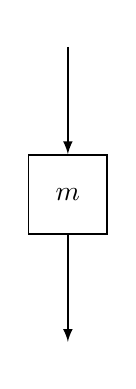
\begin{tikzpicture}[-latex ,auto ,node distance =2 cm and 2cm ,on grid ,
  semithick ,
  state/.style ={ rectangle, top color = white, bottom color = white,
  draw, black, text = black, minimum width = 1 cm, minimum height = 1 cm},
  state_invisible/.style ={ rectangle, top color = white, bottom color = white,
  draw, black, text = black, minimum width = 0.1 cm, minimum height = 0.1 cm}]]
  \node[state] (C)
  {$m$};
  \node[state_invisible, draw = none] (A) [above=of C] {};
  \node[state_invisible, draw = none] (B) [below=of C] {};
  \path (A) edge [] node[] {} (C);
  \path (C) edge [] node[] {} (B);
  \end{tikzpicture}
  \captionof{figure}{$M$-node}
  \label{fig:M1}
\end{minipage}%
\begin{minipage}{.5\textwidth}
  \centering
  \begin {tikzpicture}[-latex ,auto ,node distance =2 cm and 2cm ,on grid ,
  semithick ,
  state/.style ={ diamond, top color = white, bottom color = white,
  draw, black, text = black, minimum width = 1 cm, minimum height = 1 cm},
  state_invisible/.style ={ rectangle, top color = white, bottom color = white,
  draw, black, text = black, minimum width = 0.1 cm, minimum height = 0.1 cm}]]
  \node[state] (C)
  {$c$};
  \node[state_invisible, draw = none] (A) [above=of C] {};
  \node[state_invisible, draw = none] (B) [below=of C] {};
  \node[state_invisible, draw = none] (D) [right=of C] {};
  \path (A) edge [] node[] {} (C);
  \path (C) edge [] node[] {$\texttt{true}$} (B);
  \path (C) edge [] node[] {$\texttt{false}$} (D);
  \end{tikzpicture}
  \captionof{figure}{$C$-node}
  \label{fig:M1}
\end{minipage}
\begin{minipage}{.5\textwidth}
  \centering
  \begin {tikzpicture}[-latex, auto, node distance =2 cm and 2 cm ,on grid ,
  semithick,
  state/.style ={ circle, top color = white, bottom color = white,
  draw, black, text = black, minimum width = 1 cm, minimum height = 1 cm},
  state_invisible/.style ={ rectangle, top color = white, bottom color = white,
  draw, black, text = black, minimum width = 0.1 cm, minimum height = 0.1 cm}]]
  \node[state] (C)
  {$\texttt{HALT}$};
  \node[state_invisible, draw = none] (A) [above=of C] {};
  \path (A) edge [] node[] {} (C);
  \end{tikzpicture}
  \captionof{figure}{\texttt{HALT}-node}
  \label{fig:M1}
\end{minipage}
\end{figure}

\subsection{Evaluation Semantics}

Let $Q$ be the set of nodes for some control flow graph.  We define the set of control flow graph eval formulas for that graph as follows:

\begin{enumerate}
\item Every member of $S$ is a control flow graph eval formula.
\item If $s$ is a member of $S$ and $q$ is a member of $Q$, then $\texttt{eval}_{\texttt{cfg}}(s, q)$ is a control flow graph eval formula.
\end{enumerate}

Let $q_{\texttt{HALT}}$ denote the \texttt{HALT} state.  Then evaluation is dictated by the following reduction system:

\begin{description}
\item[IfTrueCfg] If $q$ is a $C$-node labeled with $c$, $\delta_{C}(c, s) = \texttt{true}$, and $q$ is connected to $q'$ with an edge labeled \texttt{true}, then $\texttt{eval}_{\texttt{cfg}}(s, q) \longrightarrow \texttt{eval}_{\texttt{cfg}}(s, q')$.
\item[IfFalseCfg] If $q$ is a $C$-node labeled with $c$, $\delta_{C}(c, s) = \texttt{false}$, and $q$ is connected to $q'$ with an edge labeled \texttt{false}, then $\texttt{eval}_{\texttt{cfg}}(s, q) \longrightarrow \texttt{eval}_{\texttt{cfg}}(s, q')$.
\item[MApplCfg] If $q$ is an $M$-node labeled with $m$, and $q$ is connected to $q'$, then $\texttt{eval}_{\texttt{cfg}}(s, q) \longrightarrow \texttt{eval}_{\texttt{cfg}}(\delta_{M}(m, s), q')$.
\item[HaltCfg] $\texttt{eval}_{\texttt{cfg}}(s, q_{\texttt{HALT}}) \longrightarrow s$
\end{description}

If $q_{0}$ denotes the initial state, evaluation on a state $s$ in $S$ is done by starting with the formula $\texttt{eval}_{\texttt{cfg}}(s, q_{0})$ and applying reductions until a normal form is reached.  We will now show that this evaluation is deterministic, and if it terminates, it terminates with a member of $S$.

\newtheorem*{evalcfgnormalforms}{Theorem}
\begin{evalnormalforms}
The normal forms in control flow graph evaluation are exactly the members of $S$.
\end{evalnormalforms}

\begin{proof}
(TODO: Do proof)
\end{proof}

\newtheorem*{evalcfgdeterminism}{Theorem}
\begin{evaldeterminism}
Control flow graph evaluation is deterministic.
\end{evaldeterminism}

\begin{proof}
(TODO: Do proof)
\end{proof}

\begin{comment}
%this is true, but not sure if we want/need to have this here...
\newtheorem*{evalcfgnotnormalizing}{Theorem}
\begin{evalnotnormalizing}
Evaluation is not generally normalizing.
\end{evalnotnormalizing}

\begin{proof}
(TODO: Do proof)
\end{proof}
\end{comment}

\section{Equivalence of Branch Back Program Formulas and Program Control Graphs}

It turns out to be true that the semantic spaces for Branch Back Program Formulas and Program Control Graphs are identical.  To prove this, we will show that for every (closed) Branch Back program formula, there exists a semantically equivalent program control graph, and for every program control graph, there exists a semantically equivalent (closed) Branch Back program formula.

\subsection{Branch Back Program Formulas to Control Flow Graphs}

(TODO: Do this.  The key insight is that the reduction systems are very similar, need to think about the best way to do this.)

\subsection{Control Flow Graphs to Branch Back Program Formulas}

(TODO: Do this.  We will use an equational approach here.)

\section{Conclusion}

(TODO: Some conclusion here)

\end{document}
